\chapter{Diffusive Shock Acceleration} \label{A3_DSA}

At Earth, the energy spectrum of cosmic rays have been measured up to $10^{20}~\eV$ (see \autoref{sec:chapter_1_cr_spectrum}). But how do cosmic rays reach these enormous energies? Fermi, in 1949, proposed a mechanism where cosmic rays are accelerated through the interaction with magnetic field irregularities in ISM gas clouds \citep{1949PhRv...75.1169F}. However, the amount of energy gained through these interactions was relatively small to explain the highest energy cosmic rays observed at Earth. Fermi's original theory was modified in the 1970's to consider the acceleration of cosmic rays as they travel through a shock wave generated by, for example, a SNR \citep{1977DoSSR.234.1306K,1977ICRC...11..132A,1978MNRAS.182..147B,1978MNRAS.182..443B,1978ApJ...221L..29B}. This is known as diffusive shock acceleration.

\section{Fermi's Original Theory}

In Fermi's original theory, a cosmic ray with energy $E_1$  scatters of a ISM gas cloud (travelling at velocity $v_c$ in the lab frame) at angle $\theta_1$ (see \autoref{fig:A3_DSA_fermi_orig_frames}) and exits the cloud with energy $E_2$ and angle $\theta_2$. Using Lorentz transformations, the original energy in the cloud frame (primed frame) is given by:

\begin{figure}[h!]
    \centering
    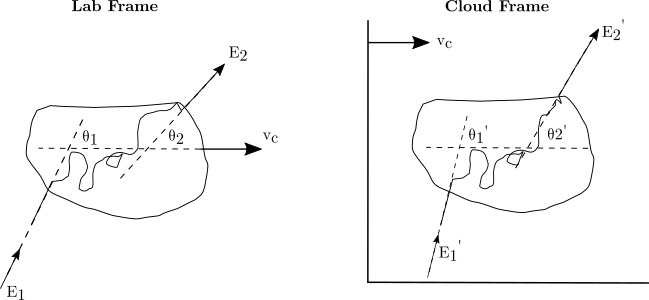
\includegraphics{A3_Diffusive_Shock_Acceleration/Images/fermi_original_theory_frames.png}
    \caption{In the lab frame (\textit{left}), a Cosmic ray with energy $E_1$ enters a ISM cloud (travelling at spped $v_c$) at angle $\theta_1$ and scatters off magnetic field tubulence and exits the cloud with energy $E_2$ and angle $\theta_2$. The same process is shown in the right, but in the reference frame of the cloud (labeled as primed).}
    \label{fig:A3_DSA_fermi_orig_frames}
\end{figure}

\begin{equation}
    \begin{aligned}
        E_1'=\gamma_cE_1\qty(1-\beta_c\cos\theta_1)\text{ ,}
    \end{aligned}
\end{equation}
\noindent where $\beta_c=v_c/c$ and $\gamma_c=1/\sqrt{1-\beta_c^2}$. The scattering is collisionless (elastic) in the reference frame of the cloud, giving $E_1'=E_2'$. The final energy in the lab frame is then:

\begin{equation}
    \begin{aligned}
        E_2&=\gamma_c E_2'\qty(1+\beta_c\cos\theta_2') \\
        &=\gamma_c^2E_1\qty(1+\beta_c\cos\theta_2')\qty(1-\beta_c\cos\theta_1) \text{ .}
    \end{aligned}
\end{equation}
\noindent The cosmic-ray fractional energy gain is then:

\begin{equation}
    \begin{aligned}
        \frac{\Delta E}{E}&=\frac{E_2-E_1}{E_1} \\
        &=\frac{1-\beta_c\cos\theta_1+\beta_c\cos\theta_1+\beta_c^2\cos\theta_1\cos\theta_2'}{\qty(1-\beta_c^2)}-1\text{ .}
    \end{aligned} \label{eq:A3_DSA_fermi_orig_frac_energy}
\end{equation}
\noindent Considering the average fractional energy gain ($\langle \Delta E/E \rangle$), the outcoing direction of the cosmic ray in the clouds reference frame is randomised, therefore $\langle \cos\theta_2'=0 \rangle$. To calculate the average original cosmic-ray angle, consider the ISM cloud traveling a distance $v_ct$ in a `sea' of cosmic rays travelling at speed $v_\text{CR}$ (see \autoref{fig:A3_fermi_origin_theta1}). In time $t$, all cosmic rays in length $l$ will enter the cloud. For relativistic cosmic rays ($v_\text{cr}>>v_c$):
\begin{SCfigure}[2.3][h]
    \centering
    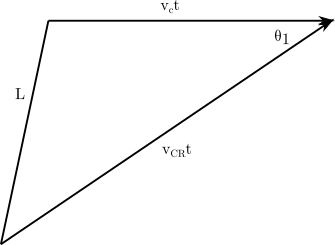
\includegraphics[width=0.3\textwidth]{A3_Diffusive_Shock_Acceleration/Images/fermi_original_theta1.png}
    \caption{A ISM cloud travelling at speed $v_c$ in a `sea' of cosmic rays. In time $t$, the cosmic rays in path $L$ with speed $v_\text{CR}$ will enter the cloud.}
    \label{fig:A3_fermi_origin_theta1}
\end{SCfigure}
\begin{equation}
    \begin{aligned}
        L&=t\sqrt{v_\text{CR}^2+v_c^2-2v_\text{CR}v_c\cos\theta_1} \\
        &\approx t\qty(v_\text{CR}-v_c\cos\theta_1) \text{ .}
    \end{aligned}
\end{equation}
\noindent For a spherical cloud of radius $r$ having cross section $\sigma=\pi r^2$, the collision rate, $R$, is:

\begin{equation}
    \begin{aligned}
        R&=\frac{n_\text{CR}L\sigma}{t} \\
        &=n_\text{CR}\sigma\qty(v_\text{CR}-v_c\cos\theta_1) \text { ,}
    \end{aligned}
\end{equation}
\noindent where $n_\text{CR}$ is the cosmic-ray density. For an isotropic cosmic-ray distribution, $\dd{n_\text{CR}}/\dd{\cos\theta_1}=n_\text{CR}/2$ for $-1<\cos\theta_1<1$, the collision rate is described by:

\begin{equation}
    \begin{aligned}
        R&=\frac{n_\text{CR}L\sigma}{t} \\
        &=\frac{n_\text{CR}\sigma}{2}\int_{-1}^1\dd{\cos\theta_1}\qty(v_\text{CR}-v_c\cos\theta_1) \text{ .}
    \end{aligned}
\end{equation}
\noindent giving the probability distribution of collision at angle $\theta_1$ to be $p_\text{coll}\propto \qty(1-\beta_c)$ for relativistic cosmic rays. The average value of $\cos\theta_1$ is then:

\begin{equation}
    \begin{aligned}
        \langle \cos\theta_1\rangle &=\frac{\int_{-1}^1\dd{\cos\theta_1}p_\text{coll}\cos\theta_1}{\int_{-1}^1\dd{\cos\theta_1}p_\text{coll}} \\
        &=-\frac{\beta}{3} \text{ .}
    \end{aligned} \label{eq:A3_DSA_fermi_orig_av_theta1}
\end{equation} 
\noindent Combining \autoref{eq:A3_DSA_fermi_orig_frac_energy}, \autoref{eq:A3_DSA_fermi_orig_av_theta1} and that $\langle \cos\theta_1 \rangle=0$:

\begin{equation}
    \begin{aligned}
        \langle \frac{\Delta E}{E} \rangle&=\frac{1-\beta_c\langle\cos\theta_1\rangle+\beta_c\cos\langle\theta_1\rangle+\beta_c^2\langle\cos\theta_1\rangle\langle\cos\theta_2'\rangle}{\qty(1-\beta_c^2)} \\
        &= \frac{4}{3}\beta_c^2 \text{ .}
    \end{aligned}
\end{equation}
\noindent The average fractional energy gain is positive and second-order in $\beta_c$ (fermi's original theory is also known as second-order Fermi acceleration). ISM gas clouds have velocity $\approx 15~\kmpersec$, resulting in a small fractional energy gain that cannot explain the highest energy cosmic rays observed at Earth. \citep{1949PhRv...75.1169F}. 

\section{Diffusive Shock Acceleration}

Diffusive shock acceleration is a modified version of Fermi's original theory that considers acceleration at a shock front (e.g. SNR shock front.)
\begin{SCfigure}[0.5][h]
	\centering
	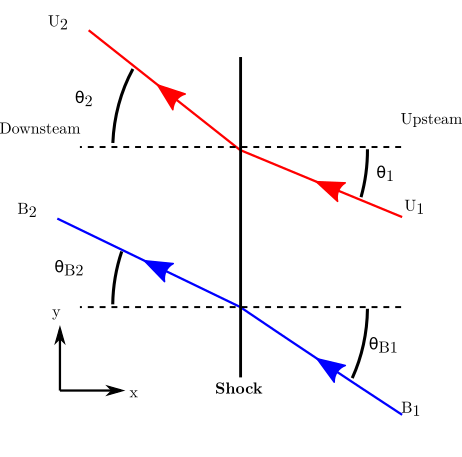
\includegraphics[width=0.7\textwidth]{A3_Diffusive_Shock_Acceleration/Images/shock_dynamics.png}
	\caption{A cosmic ray travels upstream of the shock at velocity $U_1$ (relative to the shock) at angle $\Theta_1$ and `passes` through the shock downstream. The cosmic ray now has velocity $U_2$ at angle $\Theta_2$. $B_1$ and $B_2$ are the magnetic fields upstream and downstream of the shock with angles $\theta_{B1}$ and $\theta_{B2}$ to the normal to the shock respectively.}
	\label{fig:A3_shock_dynamics}
\end{SCfigure}
\par 
A cosmic ray travelling upstream of the shock at velocity $U_1$ and angle $\theta_1$ will `pass' through the shock and travel at velocity $U_2$ and angle $\theta_2$ downstream of the shock (see \autoref{fig:A3_shock_dynamics}). The magnetic fields upstream and downstream of the shock are $B_1$ and $B_2$ respectively and $x$ and $y$ are the direction perpindicular and parallel to the shock respectively. The compression ratio is defined to be the mass density ratio of the shocked and unshocked material:

\begin{equation}
    \begin{aligned}
        r&=\frac{\rho_2}{\rho_1}\text{ ,}
    \end{aligned}
\end{equation}
\noindent where $\rho$ is the density. From conservation of mass:

\begin{equation}
    \begin{aligned}
        \rho_1U_{1x}&=\rho_2U_{2x}=A \\
        \therefore U_{1x}&=rU_{2x}\text{ ,}
    \end{aligned} \label{eq:A3_velocity_ratios}
\end{equation}
\noindent where $A$ is a constant. From conservation of momentum:

\begin{subequations}
    \begin{alignat}{1}
        U_{1y}&=U_{2y} \\
        AU_{1x}&=AU_{2x}+P\text{ ,}
    \end{alignat}
\end{subequations}
\noindent with $P$ being the pressure downstream. From the conservation of energy:

\begin{equation}
    \begin{aligned}
        \frac{1}{2}AU_{1x}^2&=\frac{1}{2}U_{2x}^2+U_{2x}\qty(E+P)\text{ ,}
    \end{aligned}
\end{equation}
\noindent it can be found that the compression ratio can be expressed in terms of the downstream internal energy $E$:

\begin{equation}
    \begin{aligned}
        r&=1+\frac{2E}{P}\text{ ,}
    \end{aligned}
\end{equation}
\noindent and $r$ takes values $4$ and $7$ for monatomic non-relativistic and relativistic gas respectively  \citep{1983RPPh...46..973D}.
\par~\par 
\begin{figure}[h]
	\centering
	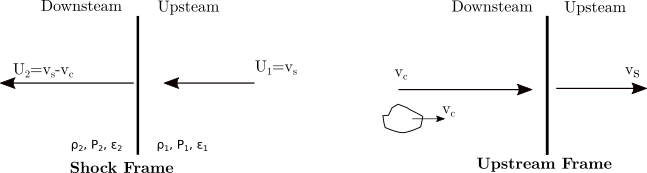
\includegraphics[width=1.0\textwidth]{A3_Diffusive_Shock_Acceleration/Images/upstream_downstream.png}
	\caption{In the reference frame of the shock (\textit{left}), a cosmic ray travels upstream of the shock (with velocity $U_{1x}$ perpindicular to the shock) to downstream of the shock (now with perpindicular velocity velocity $U_{2x})$. The same process is shown in the right, but in the upstream reference frame where the shock has velcoity $v_s$.}
	\label{fig:A3_shock_dynamics2}
\end{figure}

In the frame of the shock, the material upstream of the shock travels towards the shock at $U_1=V_s$ (see \autoref{fig:A3_shock_dynamics2}). Hence, the material downstream of the shock in the upstream reference frame (primed frame) travels at speed:

\begin{equation}
    \begin{aligned}
        U_{2x}'&=U_{1x}-U_{2x} =V_s- \frac{V_s}{r} \\
        \therefore \frac{U_{2x}'}{V_s}&=\frac{r-1}{r}\text{ ,}
    \end{aligned} \label{eq:down_upstream_v_ratio}
\end{equation}
\noindent For non-relativistic particles ${U_{2x}'}/{V_s}=3/4$.
\begin{SCfigure}[0.5][h]
	\centering
	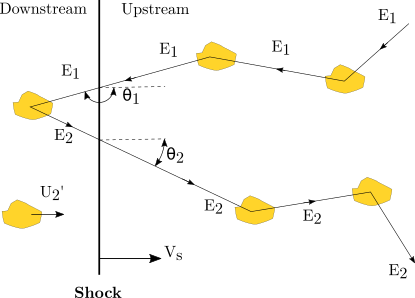
\includegraphics[width=0.65\textwidth]{A3_Diffusive_Shock_Acceleration/Images/dsa.png}
	\caption{In the reference frame of the material upstream of the shock, a cosmic ray of energy $E_1$ travels upstream to downstream with no change of energy. The cosmic ray scatters off magnetic field tubulence in a  cloud downstream of the shock and passes back upstream of the shock . This process can repeat or the cosmic ray can escape the system.}
	\label{fig:A3_shock_dynamics3}
\end{SCfigure}
\par~\par 
Now consider the scenario shown in \autoref{fig:A3_shock_dynamics3}, where a cosmic ray of energy $E_1$, velocity $v$ and angle $\theta_1$ travels upstream to downstream of the shock and scatters off a ISM cloud travelling at velocity $U_2'$. The cosmic ray, with energy $E_2$, travels back upstream at angle $\theta_2$. The rate that cosmic rays travel upstream to downstream ($u\rightarrow d$) and downstream to upstream ($d\rightarrow u$) is given by:


\begin{alignat}{2}
    R_{u\rightarrow d}\qty(\theta_1)&\approx-n_{CR}v\cos\theta_1,\quad &\ang{90}<\theta_1\ang{180} \\
    R_{d\rightarrow u}\qty(\theta_2')&\approx n_{CR}v\cos\theta_2'\quad&\ang{0}<\theta_2<\ang{90} \text{ ,}
\end{alignat}
\noindent giving the probability of crossings to be:

\begin{equation}
    \begin{aligned}
        p_{u\rightarrow d}\qty(\theta_1)&\propto -\cos\theta_1 \\
        p_{d\rightarrow u}\qty(\theta_1)&\propto \cos\theta_2  \text{ .}
    \end{aligned}
\end{equation}
\noindent Therefore, the average values of $\cos\theta_1$ and $\cos\theta_2$ are:

\begin{equation}
    \begin{aligned}
    \expectation{\cos\theta_1}&=\frac{\int_{-1}^{0} \cos\theta_1^2\dd{\cos\theta_1}}{\int_{-1}^{0}\cos\theta_1 \dd{\cos\theta_1}}=-\frac{2}{3} \\
    \expectation{\cos\theta_2'}&=\frac{\int_{0}^{1} {\cos\theta_2'}^2\dd{\cos\theta_2'}}{\int_{0}^{1}\cos\theta_2' \dd{\cos\theta_2'}}=\frac{2}{3}\text{ .}
    \end{aligned} \label{eq:A3_DSA_fermi_second_angle}
\end{equation}

\noindent Combining \autoref{eq:A3_DSA_fermi_orig_frac_energy} and \autoref{eq:A3_DSA_fermi_second_angle} gives the average fractional energy gain:

\begin{equation}
    \begin{aligned}
    \expectation{\frac{\Delta E}{E}}
	&=\frac{\beta^2+\frac{4}{3}\beta+\frac{4}{9}\beta^2}{1-\beta_\text{cloud}^2}\text{ ,}
    \end{aligned} 
\end{equation}
\noindent where $\beta=U_2'/c$. For $\beta\ll 1$:

\begin{equation}
    \begin{aligned}
    \expectation{\frac{\Delta E}{E}}
	&\approx \frac{4}{3}\beta 
    \end{aligned} 
\end{equation}
\noindent Each time the cosmic ray travels back and across the shock, the cosmic ray has increased its energy by a factor $V_s/c$. An Diffusive shock acceleration is also known as first-order fermi acceleration as the average energy gain is first order with $\beta$. 